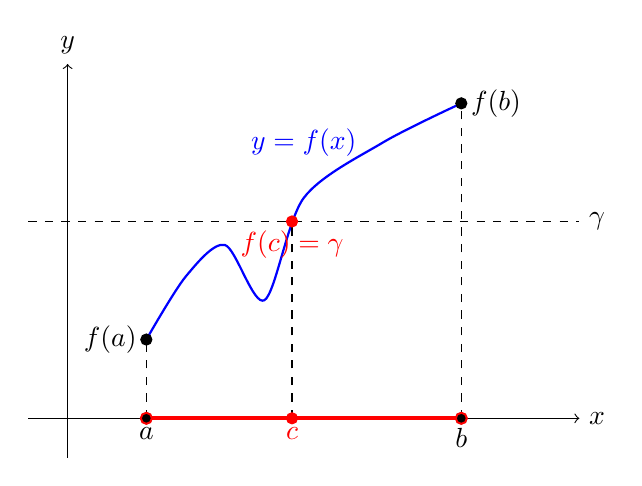
\begin{tikzpicture}[scale=1,domain=0:6,
	circledtail/.style={
		circle, draw, fill=white, inner sep=0pt, minimum size=6pt
	},
	open-open/.style={
		postaction={decorate, decoration={
				markings, 
				mark=at position 0 with {\node[circledtail]{};},  % Open circle at the start
				mark=at position 1 with {\node[circledtail]{};}   % Open circle at the end
		}}
	},
	closed-closed/.style={
		postaction={decorate, decoration={
				markings, 
				mark=at position 0 with {\filldraw[black] circle[radius=3pt];},  % Filled circle at start
				mark=at position 1 with {\filldraw[black] circle[radius=3pt];}   % Filled circle at end
		}}
	},
	open-closed/.style={
		postaction={decorate, decoration={
				markings, 
				mark=at position 0 with {\node[circledtail]{};},  % Open circle at the start
				mark=at position 1 with {\filldraw[black] circle[radius=3pt];}  % Filled circle at the end
		}},
		-{Stealth[scale=1.2]}
	},
	closed-open/.style={
		postaction={decorate, decoration={
				markings, 
				mark=at position 0 with {\filldraw[black] circle[radius=3pt];},  % Filled circle at the start
				mark=at position 1 with {\node[circledtail]{};}  % Open circle at the end
		}}
	}]
	% Draw the axes
	\draw[->] (-0.5,0) -- (6.5,0) node[right] {$x$};
	\draw[->] (0,-0.5) -- (0,4.5) node[above] {$y$};
	
	% Define points a and b on the x-axis
	\coordinate (A) at (1,0);
	\coordinate (B) at (5,0);
	
	% Define points f(a), f(b) and gamma
	\coordinate (FA) at (1,1); % f(a)
	\coordinate (FB) at (5,4); % f(b)
	\coordinate (GAMMA) at (0,2.5); % gamma horizontal line
	
	% Function graph
	\draw[color=blue,thick,smooth] plot coordinates {(1,1) (1.5,1.8) (2,2.2) (2.5,1.5) (3,2.8) (4,3.5) (5,4)};
	\node[blue] at (3,3.5) {$y=f(x)$};
		
	% Points on the graph
	\filldraw[black] (FA) circle (2pt) node[left] {$f(a)$};
	\filldraw[black] (FB) circle (2pt) node[right] {$f(b)$};
		
	% Draw vertical dashed lines for a and b
	\draw[dashed] (A) -- (FA);
	\draw[dashed] (B) -- (FB);
	
	% Labels for a and b
	\node[below] at (A) {$a$};
	\node[below] at (B) {$b$};
	
	\draw[red, line width=.5mm] (A) -- (B);
	\filldraw[black] (1,0) circle (2pt);
	\filldraw[black] (5,0) circle (2pt);
	
	% Gamma line and label
	\draw[dashed] (-0.5,2.5) -- (6.5,2.5) node[right] {$\gamma$};
	
	% Intersection point at c
	\draw[dashed] (2.85,0) -- (2.85,2.5);
	\filldraw[red] (2.85,2.5) circle (2pt) node[below] {$f(c) = \gamma$};
	\filldraw[red] (2.85,0) circle (2pt) node[below] {$c$};	
	
	\draw[red, line width = .25mm] (1,0) circle (2pt);
	\draw[red, line width = .25mm] (5,0) circle (2pt);
\end{tikzpicture}
